%%%%%%%%%%%%%%%%%%%%%%%%%%%%%%%%%%%%%%%%%%%%%%%%%%%%%%%%%%%%%%%%%%%%%%%%%%%%%%%%
%2345678901234567890123456789012345678901234567890123456789012345678901234567890
%        1         2         3         4         5         6         7         8

\documentclass[letterpaper, 10 pt, conference]{ieeeconf}  % Comment this line out if you need a4paper

%\documentclass[a4paper, 10pt, conference]{ieeeconf}      % Use this line for a4 paper

\IEEEoverridecommandlockouts                              % This command is only needed if 
                                                          % you want to use the \thanks command

\overrideIEEEmargins                                      % Needed to meet printer requirements.

% See the \addtolength command later in the file to balance the column lengths
% on the last page of the document

% The following packages can be found on http:\\www.ctan.org
\usepackage{float}
\usepackage{graphicx} % for pdf, bitmapped graphics files
%\usepackage{epsfig} % for postscript graphics files
%\usepackage{mathptmx} % assumes new font selection scheme installed
%\usepackage{times} % assumes new font selection scheme installed
%\usepackage{amsmath} % assumes amsmath package installed
%\usepackage{amssymb}  % assumes amsmath package installed

\title{\LARGE \bf
Exoskeletons
}


\author{Aydin Tekin$^{1}$% <-this % stops a space
\thanks{*This work was not supported by any organization}% <-this % stops a space
\thanks{$^{1}$Aydin Tekin is student at the Karlsruhe Institute of Technology, 76131 Karlsruhe, Germany
        {\tt\small aydin.tekin@student.kit.edu}}%
}


\begin{document}



\maketitle
\thispagestyle{empty}
\pagestyle{empty}


%%%%%%%%%%%%%%%%%%%%%%%%%%%%%%%%%%%%%%%%%%%%%%%%%%%%%%%%%%%%%%%%%%%%%%%%%%%%%%%%
\begin{abstract}

In the past twenty years the research about exoskeleton made many large steps towards the vision of a durable, natural and user-friendly exoskeleton, assisting humans in many aspects. The idea of increasing human strength or fixing weaknesses of human nature led to great efforts in making these dreams true. In this paper the current "state of art" and their key functionalities will be presented.

\end{abstract}


%%%%%%%%%%%%%%%%%%%%%%%%%%%%%%%%%%%%%%%%%%%%%%%%%%%%%%%%%%%%%%%%%%%%%%%%%%%%%%%%
\section{INTRODUCTION}

Developing exoskeletons to increase human strength and durability was firstly initiated by the US Department of Defence in the early 60's where General Electric presented the first prototype "Hardiman" which allowed the wearer to lift loads up to 750 lbs. This prototype was far away from what we today consider as an exoskeleton; one arm weighted more than 750 kg, which is thrice more weight than it could lift up.
Modern exoskeletons are designed to be user-friendly, intuitive and safe. The acceptance of the system from the eye of the user should be increased with an high amount of comfortability and agility. 



\section{STATE OF THE ART}

The different systems presented in this paper can be divided into three general types; lower body-, upper body- and full body exoskeletons.

%%%%%%%%%%%%%%%%%%%%%%%%%%%%%%%%%%%%%%%%%%%%%%%%%%%%%%%%%%%%%%%%%%%%%%%%%%%%%%%%

Lower body exoskeletons are mostly designed for the medical sector. Mostly its used for rehabilitation of people who have difficulties with walking (e.g. caused by long-term *Bett gefesselt sein* or by vestibular disorder). Some of these systems even go a step further and try to give disabled people some amount of their mobility back.

%%%%%%%%%%%%%%%%%%%%%%%%%%%%%%%%%%%%%%%%%%%%%%%%%%%%%%%%%%%%%%%%%%%%%%%%%%%%%%%%

Upper body exoskeletons have different application areas; the XOS 2 for example is planned to be used on military operations, whereas other systems aim to be used in the industry. They could be used in the entertainment industry as an addition to a VR-headset to create a even more authentic virtual reality or as an remote hand in the chemical industry to work with unsafe materials.

%%%%%%%%%%%%%%%%%%%%%%%%%%%%%%%%%%%%%%%%%%%%%%%%%%%%%%%%%%%%%%%%%%%%%%%%%%%%%%%%

The last of the three types are the full body exoskeletons, assisting the whole body. They are used mainly to lift up and transport heavy objects; for example the HULC (Human Universal Load Carrier) helps soldiers to carry more supply on the battlefield. Other systems assist people in their daily life or work.

%%%%%%%%%%%%%%%%%%%%%%%%%%%%%%%%%%%%%%%%%%%%%%%%%%%%%%%%%%%%%%%%%%%%%%%%%%%%%%%%

Altough the following systems were initially designed for a special purpose, due to continous developement, some cant be fit into just one of the mentioned types. For example the HAL (Hybring Assistive Limb) was firstly developed as lower body exoskeleton but after the second generation it was enhanced with an upper body component resulting in a full body solution. So the divison of the exoskeletons are not strict and the affinity of them might be overlap with other types.

\subsection{Lower body exoskeletons}

E-Legs was originally created by Berkeley Bionics in the USA which was later renamed to Ekso Bionics. Also the exoskeleton was relabeled to Ekso. Powered with a battery, attached at the back of the exoskeleton, it can run up to 6 hours. It is used for rehabilitation purposes, mostly for people with walking disabilities. With a self-learing algorithm adapted system control, user have to train several weeks daily, until they can independantly stand up from their wheel-chair and walk freely. Even if the system is still slow and the walking processes seems little stockingly, it gives wheel-chair confined people a great amount of mobility and freedom. This system was commercialed several years ago and is currently used/tested in rehabilitation centers but also can be bought for circa 100.000 US-Dollar.

%%%%%%%%%%%%%%%%%%%%%%%%%%%%%%%%%%%%%%%%%%%%%%%%%%%%%%%%%%%%%%%%%%%%%%%%%%%%%%%%

\begin{figure}[H]
  \centering
    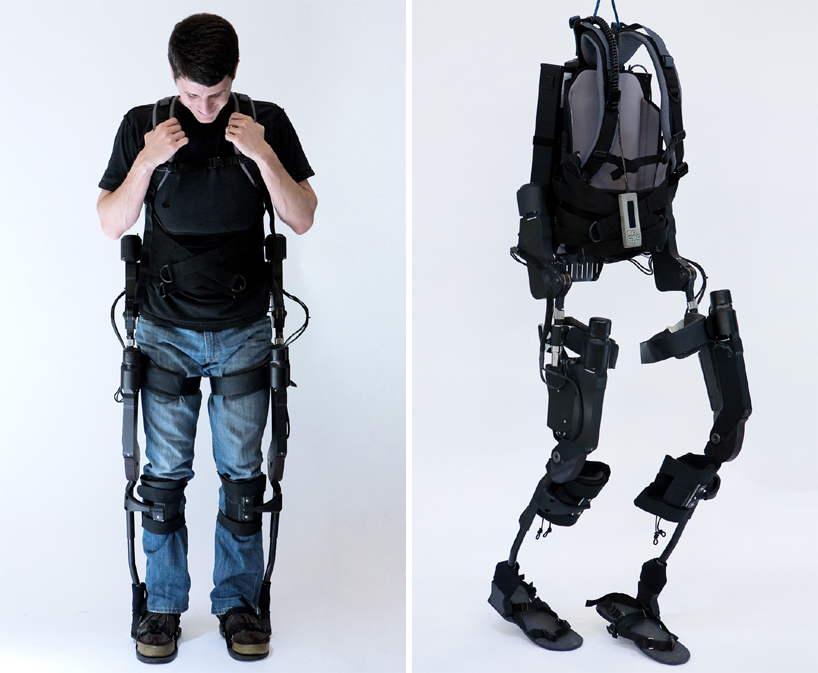
\includegraphics[width=0.5\textwidth]{img/elegs}
  \caption{HELLO}
\end{figure}

%%%%%%%%%%%%%%%%%%%%%%%%%%%%%%%%%%%%%%%%%%%%%%%%%%%%%%%%%%%%%%%%%%%%%%%%%%%%%%%%

LOPES (LOwer Powered ExoSkeleton) is being developed by the University of Twente in the Netherlands and is a stationary exoskeleton. Used also for rehabilitation like Ekso, the main difference is that this system is tethered and mostly controlled by a second operator sitting behind the computer attached to the exoskeleton. The target group are not disabled people but patients who were lost muscle mass after a long stay in hospital or people suffering vestibular disorder. The patients can be personally trained with the system which collectes data on the fly. Depending on the data, the operator can then tune the system to give the user more freedom or assist him more with the walking processes. Additionally having 8 degrees of freedom on a the legs, LOPES grants full flexibility and very natural walking flow for the user.

%%%%%%%%%%%%%%%%%%%%%%%%%%%%%%%%%%%%%%%%%%%%%%%%%%%%%%%%%%%%%%%%%%%%%%%%%%%%%%%%

\begin{figure}[H]
  \centering
    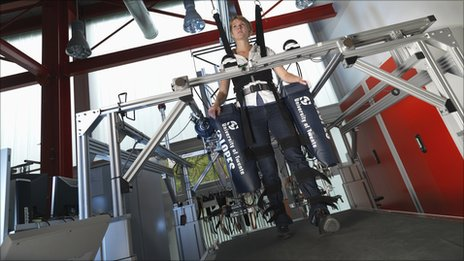
\includegraphics[width=0.5\textwidth]{img/lopes}
  \caption{HELLO}
\end{figure}

-LOPES
-Honda Walking Device

\subsection{Upper body exoskeletons}


\subsection{Full body exoskeletons}
 
Test in this test test test test test test test 
test test test test test test test test\newpage

\section{DISSCUSION}

Altough the presented systems are very advanced, there are still difficulties the researchers have to face developing efficient systems. 

%%%%%%%%%%%%%%%%%%%%%%%%%%%%%%%%%%%%%%%%%%%%%%%%%%%%%%%%%%%%%%%%%%%%%%%%%%%%%%%%

The sensor technology is still not as advanced as we think. Many systems still dont use any active sensors to to obtain human body signals, instead passive sensors measure the movement initiated by the human then try to estimate the future movement and then react to this. This has the advantage that you can easily put on the exoskeleton without having to place sensors accuratetly on defined spots on your body. But the kind of sensor system is very inaccurate and reacts pretty slowly to human interaction, which may restrict the agility of the user. Some systems use Electromyography, detecting eletrical potential generated by muscels, using EMG-Sensors on the skin of the user to analyse the movement of him. Even if we get much better results, they are still very inaccurate because we cant "dock" directly on the muscle cells. Additionally it is very difficult for a normal user to put on these kind of exoskeletons because you need an experienced assistant to put the sensors to the right spot on the body. Any deviantions could have an immense influence of the algorithm used for motion detection. Currently researchers are trying to optimize the existing sensors but also are working on other ways to obtain human signals like using EMG-needles.

%%%%%%%%%%%%%%%%%%%%%%%%%%%%%%%%%%%%%%%%%%%%%%%%%%%%%%%%%%%%%%%%%%%%%%%%%%%%%%%%

Security is also seen as an important feature in developing such systems. People who use this system must be able to trust them and the system should be "secure" otherwise the user could get injured in many ways. In the worst case the exoskeleton may wrench extremities of humans or could suddenly shutdown leaving the user back with a heavy load. That's why the researcher try to define guidelines for secure systems; one of them is ISO 13485. It covers different aspects of secure medical systems like corrective and preventive actions or risk management. HAL-5 is the first exoskeleton who has this certification and other systems are expected to follow.

%%%%%%%%%%%%%%%%%%%%%%%%%%%%%%%%%%%%%%%%%%%%%%%%%%%%%%%%%%%%%%%%%%%%%%%%%%%%%%%%

Most focus on the recent work is the question which power supply should be used and how it can be optimized. Some systems like XOS dont even use any autonomous power supplies, they are attached with wires to a station. This gives a full electrical durability but they can only be used stationary. For independant exoskeletons there are currently two different types of power supplies; the first one is using a battery which is attached to the exoskeleton. This solution has a very low capacity, so the systems can only work for a few hours which might be a very short length of time, depending on the use-case. Also batteries are heavy, recharging takes too much time and the durability of a battery decreases over time. Fuels are an alternative which can trump with a high and long-lasting energy output resulting in operating time of several days. Refilling can be done very fast and you dont have to find fixed stations to refill the energy source. But it also has its downsides, it's very noisy to use and very insecure: the content is highly flammable. The HAL-5 uses a highly optimized battery and can work up to 5 hours with one charge, using it in an medical environment there is no way to use noisy and smoking energy sources. HULC is planned to use a fuel based power supply, its important for these kind of military-used exoskeletons to have a large operation time. Until there is no other good alternative, one of the mentioned types have to be used and the disadvantes have to be accepted.
 

\section{CONCLUSION}

The human body has flaws and limitations which will and have to be fixed with the increasing technical possibilites we have. With exoskeletons, it seems like a solution for this problem is found, so the work on improving must be intensified.

%%%%%%%%%%%%%%%%%%%%%%%%%%%%%%%%%%%%%%%%%%%%%%%%%%%%%%%%%%%%%%%%%%%%%%%%%%%%%%%%

Companies understood the importance of this sector and started commercializing products, which to then just were seen as objects in research. Evermore exoskeletons are made accessible to the general public this way, even if the prices are still too high for the most people to buy them.

%%%%%%%%%%%%%%%%%%%%%%%%%%%%%%%%%%%%%%%%%%%%%%%%%%%%%%%%%%%%%%%%%%%%%%%%%%%%%%%%

The vision of a world where people use exoskeletons in their daily life or in work is not that far away then we think; some obstacles must be overcame but the recent progresses showed us that we have the needed potential to realise this vision.

\addtolength{\textheight}{-12cm}   % This command serves to balance the column lengths
                                  % on the last page of the document manually. It shortens
                                  % the textheight of the last page by a suitable amount.
                                  % This command does not take effect until the next page
                                  % so it should come on the page before the last. Make
                                  % sure that you do not shorten the textheight too much.

%%%%%%%%%%%%%%%%%%%%%%%%%%%%%%%%%%%%%%%%%%%%%%%%%%%%%%%%%%%%%%%%%%%%%%%%%%%%%%%%



%%%%%%%%%%%%%%%%%%%%%%%%%%%%%%%%%%%%%%%%%%%%%%%%%%%%%%%%%%%%%%%%%%%%%%%%%%%%%%%%



%%%%%%%%%%%%%%%%%%%%%%%%%%%%%%%%%%%%%%%%%%%%%%%%%%%%%%%%%%%%%%%%%%%%%%%%%%%%%%%%



\begin{thebibliography}{99}

\bibitem{c1} G. O. Young, �Synthetic structure of industrial plastics (Book style with paper title and editor),� 	in Plastics, 2nd ed. vol. 3, J. Peters, Ed.  New York: McGraw-Hill, 1964, pp. 15�64.
\bibitem{c2} W.-K. Chen, Linear Networks and Systems (Book style).	Belmont, CA: Wadsworth, 1993, pp. 123�135.
\bibitem{c3} H. Poor, An Introduction to Signal Detection and Estimation.   New York: Springer-Verlag, 1985, ch. 4.
\bibitem{c4} B. Smith, �An approach to graphs of linear forms (Unpublished work style),� unpublished.
\bibitem{c5} E. H. Miller, �A note on reflector arrays (Periodical style�Accepted for publication),� IEEE Trans. Antennas Propagat., to be publised.
\bibitem{c6} J. Wang, �Fundamentals of erbium-doped fiber amplifiers arrays (Periodical style�Submitted for publication),� IEEE J. Quantum Electron., submitted for publication.
\bibitem{c7} C. J. Kaufman, Rocky Mountain Research Lab., Boulder, CO, private communication, May 1995.
\bibitem{c8} Y. Yorozu, M. Hirano, K. Oka, and Y. Tagawa, �Electron spectroscopy studies on magneto-optical media and plastic substrate interfaces(Translation Journals style),� IEEE Transl. J. Magn.Jpn., vol. 2, Aug. 1987, pp. 740�741 [Dig. 9th Annu. Conf. Magnetics Japan, 1982, p. 301].
\bibitem{c9} M. Young, The Techincal Writers Handbook.  Mill Valley, CA: University Science, 1989.
\bibitem{c10} J. U. Duncombe, �Infrared navigation�Part I: An assessment of feasibility (Periodical style),� IEEE Trans. Electron Devices, vol. ED-11, pp. 34�39, Jan. 1959.
\bibitem{c11} S. Chen, B. Mulgrew, and P. M. Grant, �A clustering technique for digital communications channel equalization using radial basis function networks,� IEEE Trans. Neural Networks, vol. 4, pp. 570�578, July 1993.
\bibitem{c12} R. W. Lucky, �Automatic equalization for digital communication,� Bell Syst. Tech. J., vol. 44, no. 4, pp. 547�588, Apr. 1965.
\bibitem{c13} S. P. Bingulac, �On the compatibility of adaptive controllers (Published Conference Proceedings style),� in Proc. 4th Annu. Allerton Conf. Circuits and Systems Theory, New York, 1994, pp. 8�16.
\bibitem{c14} G. R. Faulhaber, �Design of service systems with priority reservation,� in Conf. Rec. 1995 IEEE Int. Conf. Communications, pp. 3�8.
\bibitem{c15} W. D. Doyle, �Magnetization reversal in films with biaxial anisotropy,� in 1987 Proc. INTERMAG Conf., pp. 2.2-1�2.2-6.
\bibitem{c16} G. W. Juette and L. E. Zeffanella, �Radio noise currents n short sections on bundle conductors (Presented Conference Paper style),� presented at the IEEE Summer power Meeting, Dallas, TX, June 22�27, 1990, Paper 90 SM 690-0 PWRS.
\bibitem{c17} J. G. Kreifeldt, �An analysis of surface-detected EMG as an amplitude-modulated noise,� presented at the 1989 Int. Conf. Medicine and Biological Engineering, Chicago, IL.
\bibitem{c18} J. Williams, �Narrow-band analyzer (Thesis or Dissertation style),� Ph.D. dissertation, Dept. Elect. Eng., Harvard Univ., Cambridge, MA, 1993. 
\bibitem{c19} N. Kawasaki, �Parametric study of thermal and chemical nonequilibrium nozzle flow,� M.S. thesis, Dept. Electron. Eng., Osaka Univ., Osaka, Japan, 1993.
\bibitem{c20} J. P. Wilkinson, �Nonlinear resonant circuit devices (Patent style),� U.S. Patent 3 624 12, July 16, 1990. 






\end{thebibliography}




\end{document}
